\ifx\wholebook\relax \else
% ------------------------

\documentclass{ctexart}
\usepackage[cn]{../../../prelude}

\setcounter{page}{1}

\begin{document}

%--------------------------

% ================================================================
%                 COVER PAGE
% ================================================================

\title{二叉搜索树,数据结构中的`hello world'}

\author{刘新宇
\thanks{{\bfseries 刘新宇} \newline
  Email: liuxinyu95@gmail.com \newline}
  }

\maketitle
\fi

\markboth{二叉搜索树}{初等算法}

\ifx\wholebook\relax
\chapter{二叉搜索树,数据结构中的`hello world'}
\numberwithin{Exercise}{chapter}
\fi

% ================================================================
%                 Introduction
% ================================================================
%\section{简介}

数组和链表通常被认为是最简单的“hello world”数据结构,其实它们并不简单。在某些系统中,数组是最基本的组件,甚至链表也可以由数组来实现(《算法导论》第10.3节\cite{CLRS})。另一方面,在某些函数式环境中,链表被作为最基本的组件来实现数组和其他更复杂的数据结构。

考虑这些因素,我们使用二叉搜索树(BST)作为数据结构中的“hello world”。Jon Bentley在他的《编程珠玑》一书中,曾给了这样一个有趣的题目\cite{Bentley}:如何统计一段文字中每个单词出现的次数?下面的C++程序展示了一个解法。\index{统计单词}

\lstset{language=C++}
\begin{lstlisting}
int main(int, char** ) {
    map<string, int> dict;
    string s;
    while(cin>>s)
        ++dict[s];
    map<string, int>::iterator it=dict.begin();
    for(; it!=dict.end(); ++it)
        cout<<it->first<<": "<<it->second<<"\n";
}
\end{lstlisting}

我们可以运行下面的UNIX命令获得对单词的统计结果。\footnote{在Windows系统中,相应的用法为:\texttt{type bbe.txt | wordcount.exe > wc.txt}}

\begin{verbatim}
$ g++ wordcount.cpp -o wordcount
$ cat bbe.txt | ./wordcount > wc.txt
\end{verbatim}

C++标准库中提供的\texttt{map}是一种用平衡二叉树实现的字典数据结构。例子中用单词作为key,用单词出现的次数作为值。这个程序运行快速,展示了二叉搜索树的强大功能。本章我们介绍二叉搜索树的实现,然后在后面的章节中讨论如何保证二叉树的平衡。

\section{定义}
\label{introduction} \index{二叉搜索树}

在正式开始前,我们先介绍一下广义二叉树的定义。二叉搜索树只不过是一种特殊的二叉树,我们可以递归地定义二叉树如下\index{二叉树}:

一个二叉树
\begin{itemize}
\item 或者为空,
\item 或者包含三个部分:一个值,一个左侧分支和一个右侧分支,并且这两个分支也都是二叉树。
\end{itemize}

左右分支也被称为左子树和右子树,或统称为孩子。一棵树也被称为一个节点。节点中的值可以是任何类型,甚至为空。如果一个节点的左右子树都为空,我们称之为叶子节点,否则称为分支节点。图\ref{fig:binary-tree-example}展示了二叉树的概念和例子。

\begin{figure}[htbp]
  \centering
  \subcaptionbox{二叉树的概念}{\includegraphics[scale=0.5]{img/lvr.ps}} \\
  \subcaptionbox{一棵二叉树}{\includegraphics[scale=0.5]{img/btexample.ps}}
  \caption{二叉树的概念和例子}
  \label{fig:binary-tree-example}
\end{figure}

一棵二叉搜索树是一棵满足下面条件的二叉树:
\begin{itemize}
\item 所有左侧分支的值都小于本节点的值,
\item 本节点的值小于所有右侧分支的值。
\end{itemize}

图\ref{fig:bst-example}展示了一个二叉搜索树的例子。和图\ref{fig:binary-tree-example}比较,可以看到节点的组织方式是不同的。一个广义二叉树的值可以是任意类型,而二叉搜索树的定义要求它的值必须能比较大小\footnote{实际上只要能进行小于比较就足够了。}。为了强调这种区别,我们特别称二叉搜索树的的值为键(key),把节点存储的其他数据信息称为值(value)。

\begin{figure}[htbp]
  \centering
  \includegraphics[scale=0.5]{img/bst-1.ps}
  \caption{二叉搜索树的例子} \label{fig:bst-example}
\end{figure}


% ================================================================
% Data layout
% ================================================================
\section{数据组织}
\index{二叉搜索树!数据组织}

根据二叉搜索树的定义,在传统的命令式编程环境中,我们可以用指针来描绘数据的组织结构。如图\ref{fig:node-layout-parent}。

%\begin{figure}[htbp]
%       \begin{center}
%        \includegraphics[scale=0.8]{img/node-layout.ps}
%        \caption{Node layout.} \label{fig:node-layout}
%       \end{center}
%\end{figure}

一个树的节点首先包含一个键,一个键可以附加一些额外的数据(也称为“satellite data”)。接下来分别是指向左右子树的两个指针。为了方便从一个节点上溯到祖先节点,有时也在节点上存储一个指向父亲的指针(称为“父指针”)。
%Figure \ref{fig:node-layout-parent} shows the layout with parent field.

\begin{figure}[htbp]
  \centering
  \includegraphics[scale=0.8]{img/node-layout-parent.ps}
  \caption{带有父指针的数据组织结构} \label{fig:node-layout-parent}
\end{figure}

本章中,我们在讨论中有时会忽略“satellite data”以简化问题。下面的C++例子代码依据上面的数据的组织方式定义了二叉搜索树的节点。

\lstset{language=C++, commentstyle=\rmfamily, texcl=true}
\begin{lstlisting}
template<class T>
struct node {
    node(T x):key(x), left(0), right(0), parent(0){}
    ~node() {
        delete left;
        delete right;
    }

    node* left;
    node* right;
    node* parent; //可选,方便succ和pred操作
    T key;
};
\end{lstlisting}

在以链表作为基本数据结构的环境中,例如Lisp,二叉搜索树也可以由链表来构建,如图\ref{fig:lisp-layout}。

\begin{figure}[htbp]
  \centering
  \includegraphics[scale=0.8]{img/lisp-layout.ps}
  \caption{由链表构件的二叉搜索树。其中\texttt{left...}和\texttt{right...}或者为空,或者是以同样方式构建的节点。}
  \label{fig:lisp-layout}
\end{figure}

在许多函数式环境中,难以用指针来进行回溯(通常以自顶向下的递归来代替回溯),所以在数据组织上往往不使用“父节点”。

为了简化问题,我们在此后将跳过这样的具体数据组织细节,而只关注数据结构的逻辑。例如,下面的Haskell代码定义了二叉搜索树的节点。

\begin{lstlisting}[style=Haskell]
data Tree a = Empty
            | Node (Tree a) a (Tree a)
\end{lstlisting}

% ================================================================
% Insert
% ================================================================
\section{插入}
\index{二叉搜索树!插入}

我们可以使用下述算法向一个二叉搜索树中插入一个键$k$(在实际应用中,有时会同时插入一对键和值):

\begin{itemize}
\item 如果树为空,创建一个叶子节点,令该节点的key = $k$;
\item 如果$k$小于根节点的key,将它插入到左子树中;
\item 如果$k$大于根节点的key,将它插入到右子树中。
\end{itemize}

这里存在一个特殊情况,当$k$等于根节点的key时,说明它已经存在了。我们可以覆盖(overwrite)掉以前的数据,也可以选择跳过不做任何处理。简单起见,我们忽略这一情况。

插入算法是递归的。它十分简单,因此我们说二叉搜索树是“hello world”数据结构。这一算法可以形式化地定义为如下的函数。

\be
insert(T, k) = \left \{
  \begin{array}
  {r@{\quad:\quad}l}
  node(\phi, k, \phi) & T = \phi \\
  node(insert(T_l, k), k', T_r) & k < k' \\
  node(T_l, k', insert(T_r, k)) & otherwise
  \end{array}
\right.
\ee

其中,当$T$不为空时,$T_l$, $T_r$和$k'$分别是它的左右子树和key。函数$node$以给定的左子树、key和右子树为参数创建一个新节点。符号$\phi$表示NIL或空。

将上述函数直接翻译为Haskell代码可以得到下面的程序:

\begin{lstlisting}[style=Haskell]
insert Empty k = Node Empty k Empty
insert (Node l x r) k | k < x = Node (insert l k) x r
                      | otherwise = Node l x (insert r k)
\end{lstlisting}

这一程序使用了语言提供的模式匹配(pattern matching)特性。但即使不用这一特性(例如Lisp方言Scheme),函数式的插入程序仍然十分简洁。

\lstset{language=lisp}
\begin{lstlisting}
(define (insert tree x)
  (cond ((null? tree) (list '() x '()))
	((< x (key tree))
	 (make-tree (insert (left tree) x)
		    (key tree)
		    (right tree)))
	((> x (key tree))
	 (make-tree (left tree)
		    (key tree)
		    (insert (right tree) x)))))
\end{lstlisting}

这一算法也可以完全不用递归,而用循环的方式实现:

\begin{algorithmic}[1]
\Function{Insert}{$T, k$}
  \State $root \gets T$
  \State $x \gets$ \Call{Create-Leaf}{$k$}
  \State $parent \gets NIL$
  \While{$T \neq NIL$}
    \State $parent \gets T$
    \If{$k <$ \Call{Key}{$T$}}
      \State $T \gets $ \Call{Left}{$T$}
    \Else
      \State $T \gets $ \Call{Right}{$T$}
    \EndIf
  \EndWhile
  \State \Call{Parent}{$x$} $\gets parent$
  \If{$parent = NIL$} \Comment{树$T$为空}
    \State \Return $x$
  \ElsIf{$k <$ \Call{Key}{$parent$}}
    \State \Call{Left}{$parent$} $\gets x$
  \Else
    \State \Call{Right}{$parent$} $\gets x$
  \EndIf
  \State \Return $root$
\EndFunction
\Statex
\Function{Create-Leaf}{k}
  \State $x \gets $ \Call{Empty-Node}{}
  \State \Call{Key}{$x$} $ \gets k$
  \State \Call{Left}{$x$} $ \gets NIL$
  \State \Call{Right}{$x$} $ \gets NIL$
  \State \Call{Parent}{$x$} $ \gets NIL$
  \State \Return $x$
\EndFunction
\end{algorithmic}

虽然没有函数式算法那样简洁,但是它的速度很快,并且可以处理深度很大的树。限于篇幅,相应完整的C++和Python程序就不再列出了。读者可以从本书的网站下载参考。

\section{遍历}
\index{二叉树!遍历}

遍历是指依次访问二叉树中的每个元素。有三种遍历方法,分别是前序遍历、中序遍历和后序遍历。它们是按照访问根节点和子节点的先后顺序命名的。

\begin{itemize}
\item 前序遍历:先访问根节点,然后访问左子树,最后访问右子树;
\item 中序遍历:先访问左子树,然后访问根节点,最后访问右子树;
\item 后序遍历:先访问左子树,然后访问右子树,最后访问根节点。
\end{itemize}

\index{前序遍历} \index{中序遍历} \index{后序遍历}

所有的“访问”操作都是递归的。\underline{先}访问根后访问子分支称为\underline{先序},在访问左右分支的\underline{中间}访问根称为\underline{中序},先访问子分支\underline{后}访问根称为\underline{后序}。

对于图\ref{fig:bst-example}中的二叉树,下面分别列出了三种遍历的结果:

\begin{itemize}
\item 前序遍历:4, 3, 1, 2, 8, 7, 16, 10, 9, 14;
\item 中序遍历:1, 2, 3, 4, 7, 8, 9, 10, 14, 16;
\item 后序遍历:2, 1, 3, 7, 9, 14, 10, 16, 8, 4。
\end{itemize}

对二叉搜索树进行中序遍历,元素就会按照从小到大的顺序输出。二叉搜索树的定义保证了这一有趣的性质,作为练习,请读者思考如何证明。

中序遍历的算法可以描述为:
\begin{itemize}
\item 如果树为空,则返回;
\item 否则先中序遍历左子树,然后访问根节点,最后再中序遍历右子树。
\end{itemize}

这一描述本身是递归的,如果二叉树非空,令$T_l$, $T_r$和$k$分别代表左右子树和key。我们可以定义下面的抽象map函数。

\be
map(f, T) = \left \{
  \begin{array}
  {r@{\quad:\quad}l}
  \phi & T = \phi \\
  node(T_l', k', T_r') & otherwise
  \end{array}
\right .
\ee

其中

\[
 \begin{array}{l}
 T_l' = map(f, T_l) \\
 T_r' = map(f, T_r) \\
 k' = f(k)
 \end{array}
\]

这一函数可以将一棵树转换成形状完全一样的另一棵树,只不过所有节点上的值都按照某个映射进行了变换。我们也可以只访问并操作节点上的值,而不去创建另外一棵树,如下面的C++程序:

\lstset{language=C++}
\begin{lstlisting}
template<class T, class F>
void in_order_walk(node<T>* t, F f) {
    if(t) {
        in_order_walk(t->left, f);
        f(t->value);
        in_order_walk(t->right, f);
    }
}
\end{lstlisting}

这一函数接受一个参数\texttt{f},它可以是一个函数指针,或者是一个函数对象。然后程序按照中序遍历依次应用(apply)f到每个元素上。

我们还可以进一步简化这一算法,通过中序遍历将一棵二叉搜索树转化为一个有序序列。

\be
toList(T) = \left \{
  \begin{array}
  {r@{\quad:\quad}l}
  \phi & T = \phi \\
  toList(T_l) \cup \{ k \} \cup toList(T_r) & otherwise
  \end{array}
\right .
\ee

下面的Haskell程序实现了这一转换函数。

\begin{lstlisting}[style=Haskell]
toList Empty = []
toList (Node l x r) = toList l ++ [x] ++ toList r
\end{lstlisting}

我们因此得到了一个排序的方法:先把一个无序的列表转化为一个二叉搜索树,然后再用中序遍历把树转换回列表。这一排序方法被称为“树排序”。记待排序列表为$X = \{x_1, x_2, x_3, ..., x_n\}$。

\be
  sort(X) = toList(fromList(X))
\ee

我们也可以写成函数组合(function composition)的形式:

\[
  sort = toList . fromList
\]

其中函数$fromList$不断地将元素从列表中插入到一棵空的二叉搜索树中。

\be
  fromList(X)= foldL(insert, \phi, X)
\ee

这一表达也可以写成部分应用(partial application)的形式\footnote{亦称为柯里化形式(Curried form),借此来纪念数学家和逻辑学家Haskell Curry。}。

\[
  fromList = foldL \quad insert \quad \phi
\]

对于不熟悉从左侧进行fold的读者,这一函数也可以递归地定义如下:

\[
fromList(X) = \left \{
  \begin{array}
  {r@{\quad:\quad}l}
  \phi & X = \phi \\
  insert(fromList(\{x_2, x_3, ..., x_n\}), x_1) & otherwise
  \end{array}
\right .
\]

我们将会大量使用fold、函数组合和部分(parital)求值的概念。读者可以参考本书的附录A或其他参考资料,如\cite{wiki-fold}、\cite{func-composition}以及\cite{curry}。

\begin{Exercise}

\begin{itemize}
\item 给定如下前序遍历和中序遍历的结果,请重建出二叉树,并给出后序遍历的结果。
\begin{itemize}
\item 前序遍历结果:1, 2, 4, 3, 5, 6;
\item 中序遍历结果:4, 2, 1, 5, 3, 6;
\item 后序遍历结果:?
\end{itemize}
\index{重建树}

\item 归纳前一题的规律,编程实现从前序遍历和中序遍历的结果重建二叉树。

\item 证明对二叉搜索树进行中序遍历可以将全部元素按照从小到大的顺序输出。

\item 使用Big-O分析树排序的算法复杂度。
\end{itemize}
\end{Exercise}

% ================================================================
% Querying a binary search tree
% ================================================================
\section{搜索}
\index{二叉搜索树!搜索}
\index{二叉搜索树!查找}

二叉搜索树有三种不同的搜索:在树中查找一个key(亦称lookup);查找最大或最小的元素;以及查找给定元素的上一个(predecessor)或下一个(successor)元素。

\subsection{lookup}
二叉搜索树的定义使得它非常适合进行元素的查找。可以按照下面描述的方法在树中查找一个key:

\begin{itemize}
\item 如果树为空,查找失败;
\item 如果根节点的key等于待查找的值,查找成功,返回根节点作为结果;
\item 如果待查找的值小于根节点的key,继续在左子树中递归查找;
\item 否则,待查找的值大于根节点的key,继续在右子树中递归查找。
\end{itemize}

这一算法可以定义为下面的递归函数,其中$T_l$,$T_r$和$k$分别为非空二叉树的左右子树和key。

\be
lookup(T, x) = \left \{
  \begin{array}
  {r@{\quad:\quad}l}
  \phi & T = \phi \\
  T & k = x \\
  lookup(T_l, x) & x < k \\
  lookup(T_r, x) & otherwise
  \end{array}
\right .
\ee

在实际应用中,我们也可以返回这一key对应的数据(satellite data)而不是整个节点。这一算法简单直观,可以直接翻译为下面的Haskell例子程序。

\begin{lstlisting}[style=Haskell]
lookup Empty _ = Empty
lookup t@(Node l k r) x | k == x = t
                        | x < k = lookup l x
                        | otherwise = lookup r x
\end{lstlisting}

如果二叉树很平衡,绝大多数节点都有非空的左右分支,对于$n$个元素的二叉树,搜索算法的性能为$O(\lg n)$。我们将在红黑树一章给出平衡的正式定义。如果二叉树很不平衡,最坏情况下,查找的时间会退化到$O(n)$。如果记树的高度为$h$,则算法的性能可以统一成$O(h)$的形式。

搜索算法也可以不使用递归来实现。

\begin{algorithmic}[1]
\Function{Lookup}{$T, x$}
  \While{$T \neq NIL \wedge$ \Call{Key}{$T$} $ \neq x$}
    \If{$x <$ \Call{Key}{$T$}}
      \State $T \gets $ \Call{Left}{$T$}
    \Else
      \State $T \gets $ \Call{Right}{$T$}
    \EndIf
  \EndWhile
  \State \Return $T$
\EndFunction
\end{algorithmic}

下面的C++程序实现了这一消除递归的算法。

\lstset{language=C++}
\begin{lstlisting}
template<class T>
node<T>* lookup(node<T>* t, T x) {
    while(t && t->key!=x) {
        if(x < t->key) t=t->left;
        else t=t->right;
    }
    return t;
}
\end{lstlisting}

\subsection{最小元素和最大元素}
\index{二叉搜索树!最小元素/最大元素}

在二叉搜索树中,较小的元素总是位于左侧分支,而较大的元素总是位于右侧分支。可以利用这一特性来获取最大元素和最小元素。

为了获取最小元素,我们可以不断向左侧前进,直到左侧分支为空。类似地,我们可以通过不断向右侧前进获取最大元素。

\be
min(T) = \left \{
  \begin{array}
  {r@{\quad:\quad}l}
  k & T_l = \phi \\
  min(T_l) & otherwise
  \end{array}
\right .
\ee

\be
max(T) = \left \{
  \begin{array}
  {r@{\quad:\quad}l}
  k & T_r = \phi \\
  max(T_r) & otherwise
  \end{array}
\right .
\ee

这两个函数的性能都是$O(h)$,其中$h$是树的高度。当二叉树比较平衡时,$min$和$max$的性能为$O(\lg n)$,最坏情况下,性能退化为$O(n)$。

为了节省篇幅,我们没有给出相应的例子程序。同样,它们也可以不使用递归而纯用循环来实现。

\subsection{前驱(Successor)和后继(predecessor)}
\index{二叉搜索树!前驱/后继}

有些情况下,需要把二叉搜索树当作通用容器,使用迭代器(iterator)进行遍历。这就需要查找一个给定元素的前驱(上一个)或后继(下一个)元素。为了方便实现,我们需要每个节点都存储它的父节点。

很难找到简单的函数式算法来寻找前驱和后继元素。这主要是因为在纯函数的环境下,没有办法使用像指针这样的概念来引用父节点\footnote{ML或OCaml语言中有\texttt{ref}(引用)概念,但是这里我们讨论纯函数式的情况。}。一种折衷的方案是在遍历树的时候,留下一些“面包屑”作为标记。它们将来可以用来回溯甚至重建整个树。这种同时包含树和“面包屑”信息的数据结构称为zipper。读者可以参考\cite{learn-haskell}的最后一章。

但是,如果仔细考虑查找前驱和后继元素的初衷:“作为一个通用容器,遍历二叉搜索树中的全部元素”,我们就会意识到,在纯函数的环境中,根本不需要查找前驱和后继。因为我们可以用前面定义的$map$函数,按照升序遍历所有元素。

在后继章节中,我们还会遇到很多仅在命令式环境中才有的问题。它们在纯函数环境中没有意义,或者根本就不是一个问题。如何在红黑树中删除一个元素就是一个典型例子\cite{okasaki-blog}。

本节中,我们只介绍如何在二叉搜索树中查找前驱和后继元素的命令式算法。

\begin{figure}[htbp]
  \centering
  \includegraphics[scale=0.45]{img/bst-1.ps}
  \caption{查找后继元素:8的后继元素为其右侧分支中的最小值9;\\
           为了获得2的后继元素,首先向上找到1,它没有左子树,所以继续向上找到3,3的左侧孩子同样是2的祖先,故而后继元素为3。} \label{fig:bst-succ}
\end{figure}

给定元素$x$,它的后继元素$y$是满足$y>x$的最小值。有两种情况:如果$x$所在的节点有一个非空的右子树,则右子树中的最小值就是答案。如图\ref{fig:bst-succ}所示,8的后继元素为9,它是元素8的右子树中的最小值。另外一种情况是,如果$x$没有非空的右子树,我们需要向上回溯,找到最近的一个祖先,使得该祖先的左侧孩子,也为$x$的祖先。如图\ref{fig:bst-succ}所示,元素2所在的节点没有右侧分支,我们向上回溯一步找到元素1,但是1没有左侧分支,因此需要继续向上查找,这次我们到达了元素3所在的节点。而3的左侧孩子,同样也是2的祖先。至此,我们找到了2的后继元素3。

我们可以给出查找后继元素的算法如下:

\begin{algorithmic}[1]
\Function{Succ}{$x$}
  \If{\Call{Right}{$x$} $\neq NIL$}
    \State \Return \textproc{Min}(\Call{Right}{$x$})
  \Else
    \State $p \gets $ \Call{Parent}{$x$}
    \While{$p \neq NIL$ and $x =$ \Call{Right}{$p$}}
      \State $x \gets p$
      \State $p \gets $ \Call{Parent}{$p$}
    \EndWhile
    \State \Return $p$
  \EndIf
\EndFunction
\end{algorithmic}

当元素$x$没有后继元素时,这一算法返回空指针NIL。寻找前驱元素的算法非常类似,它和寻找后继元素的算法是对称的。

\begin{algorithmic}[1]
\Function{Pred}{$x$}
  \If{\Call{Left}{$x$} $\neq NIL$}
    \State \Return \textproc{Max}(\Call{Left}{$x$})
  \Else
    \State $p \gets $ \Call{Parent}{$x$}
    \While{$p \neq NIL$ and $x =$ \Call{Left}{$p$}}
      \State $x \gets p$
      \State $p \gets $ \Call{Parent}{$p$}
    \EndWhile
    \State \Return $p$
  \EndIf
\EndFunction
\end{algorithmic}

下面的Python例子程序实现了前驱与后继元素的查找算法。

\lstset{language=Python}
\begin{lstlisting}
def succ(x):
    if x.right is not None: return tree_min(x.right)
    p = x.parent
    while p is not None and p.left != x:
        x = p
        p = p.parent
    return p

def pred(x):
    if x.left is not None: return tree_max(x.left)
    p = x.parent
    while p is not None and p.right != x:
        x = p
        p = p.parent
    return p
\end{lstlisting}

\begin{Exercise}

\begin{itemize}
\item 如果将树作为一个通用容器,请使用\textproc{Pred}和\textproc{Succ},来实现这个容器的迭代遍历(traverse with iterator)。这一遍历过程的算法复杂度是什么?

\item 为了遍历一个区间$[a, b]$内的元素,在C++中,这一算法可用如下代码实现:

\texttt{for\_each (m.lower\_bound(12), m.upper\_bound(26), f);}

您能找到纯函数式的方法来解决这一问题么?
\index{区间遍历}
\end{itemize}

\end{Exercise}

% ================================================================
%                 Deletion
% ================================================================
\section{删除}
\index{二叉搜索树!删除}
二叉搜索树中,删除也是一个仅在命令式环境下有意义的问题。这是因为删除操作会改变树的结构,而在纯函数的环境中,树一旦构建完成,其结构都不会再改变。

本节展示的纯函数式的删除方法本质上并没有改变树,而是重建了一棵新的树。

删除操作是二叉搜索树中最复杂的操作。这是因为,我们必须保证删除后二叉搜索树的属性不能被破坏。也就是说,对于任何节点,所有左侧分支的元素仍然小于节点的key,而所有右侧分支的元素仍然大于节点的key。不做任何额外处理的删除会破坏这一性质。

本书采用的删除算法和一些教科书(\cite{CLRS}第262-264页)中的不同,我们采用了SGI STL中的一种简单实现\cite{sgi-stl}。

从二叉搜索树中删除节点$x$的方法如下:
\begin{itemize}
\item 如果$x$没有子节点,或者只有一个孩子,直接将$x$“切下”;
\item 否则,$x$有两个孩子,我们用其右子树中的最小值替换掉$x$,然后将右子树中的这一最小值“切掉”。
\end{itemize}

这一简洁的算法使用了这样一条特性:右子树中的最小值节点不可能有两个非空的孩子。所以上面的第二种情形简化为第一种情况,因而可以直接将最小值节点“切掉”。

图\ref{fig:del-leaf}、\ref{fig:del-1child}和\ref{fig:del-branch}描述了删除节点时的各种情况。

\begin{figure}[htbp]
  \centering
  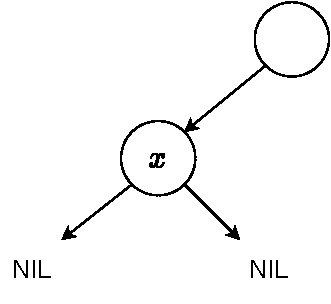
\includegraphics[scale=0.5]{img/del-leaf.ps}
  \caption{对于叶子节点,可以直接将$x$“切下”} \label{fig:del-leaf}
\end{figure}

\begin{figure}[htbp]
  \centering
  \subcaptionbox{删除$x$前}{\includegraphics[scale=0.5]{img/del-lc-before.ps}}
  \subcaptionbox{删除$x$后。$x$被“切掉”并由其左侧分支代替}{\includegraphics[scale=0.5]{img/del-lc-after.ps}} \\
  \subcaptionbox{删除$x$前}{\includegraphics[scale=0.5]{img/del-rc-before.ps}}
  \subcaptionbox{删除$x$后。$x$被“切掉”并由其右侧分支代替}{\includegraphics[scale=0.5]{img/del-rc-after.ps}}
  \caption{删除只有一个非空子分支的节点}
  \label{fig:del-1child}
\end{figure}

\begin{figure}[htbp]
  \centering
  \subcaptionbox{删除$x$前}{\includegraphics[scale=0.5]{img/del-branch-before.ps}}
  \subcaptionbox{删除$x$后。$x$被替换为右侧分支中的被“切下”的最小值}{ \includegraphics[scale=0.5]{img/del-branch-after.ps}}
  \caption{删除有两个非空分支的节点}
  \label{fig:del-branch}
\end{figure}

根据这个思路,删除操作可以定义为下面的函数。

\be
delete(T, x) = \left \{
  \begin{array}
  {r@{\quad:\quad}l}
  \phi & T = \phi \\
  node(delete(T_l, x), k, T_r) & x < k \\
  node(T_l, k, delete(T_r, x)) & x > k \\
  T_r & x = k \land T_l = \phi \\
  T_l & x = k \land T_r = \phi \\
  node(T_l, y, delete(T_r, y)) & otherwise
  \end{array}
\right .
\ee

其中,$T_l$, $T_r$, $k$分别是当$T$非空时的左右子树和key:
\[
\begin{array}{l}
T_l = left(T) \\
T_r = right(T) \\
k = key(T) \\
y = min(T_r)
\end{array}
\]

这一函数可以翻译为下面的Haskell例子程序。

\begin{lstlisting}[style=Haskell]
delete Empty _ = Empty
delete (Node l k r) x | x < k = (Node (delete l x) k r)
                      | x > k = (Node l k (delete r x))
                      -- x == k
                      | isEmpty l = r
                      | isEmpty r = l
                      | otherwise = (Node l k' (delete r k'))
                          where k' = min r
\end{lstlisting}

函数\texttt{isEmpty}用来判断一棵树是否为空($\phi$)。这一算法首先进行查找以定位到要删除的节点,然后执行删除操作。如果树的高度为$h$,则算法的复杂度为$O(h)$。

当然也可以直接传入待删除的节点,而不是key。这样就不需要先查找而可以直接进行删除。

命令式的删除算法相对更复杂一些。这是因为我们需要在删除后,把父节点(指针或引用)设置正确。下面的算法返回删除后的树。

\begin{algorithmic}[1]
\Function{Delete}{$T, x$}
  \State $r \gets T$
  \State $x' \gets x$ \Comment{保存$x$}
  \State $p \gets $ \Call{Parent}{$x$}
  \If{\Call{Left}{$x$} $= NIL$}
    \State $x \gets $ \Call{Right}{$x$}
  \ElsIf{\Call{Right}{$x$} $= NIL$}
    \State $x \gets $ \Call{Left}{$x$}
  \Else
    \Comment{两棵子树都不为空}
    \State  $y \gets $ \textproc{Min}(\Call{Right}{$x$})
    \State \Call{Key}{$x$} $\gets$ \Call{Key}{$y$}
    \State Copy other satellite data from $y$ to $x$
    \If{\Call{Parent}{$y$} $\neq x$}
      \Comment{$y$没有左子树}
      \State \textproc{Left}(\Call{Parent}{$y$}) $\gets$ \Call{Right}{$y$}
    \Else
      \Comment{$y$是$x$的右子树的根节点}
      \State \Call{Right}{$x$} $\gets$ \Call{Right}{$y$}
    \EndIf
    \If{\Call{Right}{$y$} $\neq NIL$}
      \State \textproc{Parent}(\Call{Right}{$y$}) $\gets$ \Call{Parent}{$y$}
    \EndIf
    \State Remove $y$
    \State \Return $r$
  \EndIf
  \If{$x \neq NIL$}
    \State \Call{Parent}{$x$} $\gets p$
  \EndIf
  \If{$p = NIL$}
    \Comment{删除树的根节点}
    \State $r \gets x$
  \Else
    \If{\Call{Left}{$p$} $= x'$}
      \State \Call{Left}{$p$} $\gets x$
    \Else
      \State \Call{Right}{$p$} $\gets x$
    \EndIf
  \EndIf
  \State Remove $x'$
  \State \Return $r$
\EndFunction
\end{algorithmic}

这里我们假定待删除的节点不为空(否则我们可以直接返回原先的树)。算法首先记录下树的根节点、待删除的节点和它的父节点。

如果待删除节点的任一分支为空,算法直接将$x$“切掉”。否则,如果两个分支都不为空,我们需要先在右子树中找到最小值节点$y$。用这个最小值替换掉$x$中的值,同时将附加数据(satellite data)也替换过去。最后将$y$“切掉”。注意,这里有一个特殊的情况,就是$y$本身就是$x$右子树的根节点。

我们还需要把之前保存的父节点重新设好。如果该父节点为空,则说明要删除的节点是根节点。这种情况下,我们需要返回新的根。最后,当父节点被设置好后,就可以把$x$从内存中删除了。

下面的Python程序实现了删除算法,由于Python有垃圾回收(GC)的机制,因此无需显示地回收内存。

\lstset{language=Python}
\begin{lstlisting}
def tree_delete(t, x):
    if x is None:
        return t
    [root, old_x, parent] = [t, x, x.parent]
    if x.left is None:
        x = x.right
    elif x.right is None:
        x = x.left
    else:
        y = tree_min(x.right)
        x.key = y.key
        if y.parent != x:
            y.parent.left = y.right
        else:
            x.right = y.right
        if y.right is not None:
            y.right.parent = y.parent
        return root
    if x is not None:
        x.parent = parent
    if parent is None:
        root = x
    else:
        if parent.left == old_x:
            parent.left = x
        else:
            parent.right = x
    return root
\end{lstlisting}

由于算法有可能搜索子树中的最小元素,因此对于高度为$h$的树,其复杂度为$O(h)$。

\begin{Exercise}

\begin{itemize}
\item 当节点的两个分支都不为空时,存在一种对称的删除算法:用左子树的最大值替换待删除的节点,然后将此最大值的节点“切下”。编程实现这一算法。
\end{itemize}

\end{Exercise}

\section{随机构建二叉搜索树}
\index{二叉搜索树!随机构建}

本章给出的所有算法的复杂度都依赖于二叉树的高度$h$。如果树非常不平衡,$h$就会接近$O(n)$,因此$O(h)$退化为线性复杂度。反之,如果树很平衡,$h$接近$O(\lg n)$,我们给出的这些二叉树算法的性能就会很好。

在接下来的章节中,我们会仔细讨论如何保证二叉搜索树的平衡性。但是这里可以给出一个简单的方法。如\cite{CLRS}(第265-268页)中所述,二叉搜索树可以通过随机构建来避免不平衡(严格地说是减小可能性)。也就是说,在我们构建二叉搜索树前,先通过随机函数打乱元素的次序,然后再依次把这些元素插入。

\begin{Exercise}

\begin{itemize}
\item 编程实现随机构建二叉搜索树。
\item 请读者用自己实现的二叉搜索树来统计一篇文章中各个单词出现的次数。
\item 如何在一棵二叉树中找到“距离最远”的两个节点?
\end{itemize}

\end{Exercise}

\ifx\wholebook\relax \else
\begin{thebibliography}{99}

\bibitem{CLRS}
Thomas H. Cormen, Charles E. Leiserson, Ronald L. Rivest and Clifford Stein.
``Introduction to Algorithms, Second Edition''(《算法导论》中文版). ISBN:0262032937. The MIT Press. 2001

\bibitem{Bentley}
Jon Bentley. ``Programming Pearls(2nd Edition)''(《编程珠玑》中文版). Addison-Wesley Professional; 2 edition (October 7, 1999). ISBN-13: 978-0201657883

\bibitem{okasaki-blog}
Chris Okasaki. ``Ten Years of Purely Functional Data Structures''. http://okasaki.blogspot.com/2008/02/ten-years-of-purely-functional-data.html

\bibitem{sgi-stl}
SGI. ``Standard Template Library Programmer's Guide''. http://www.sgi.com/tech/stl/

% not available any more
%\bibitem{literal-program}
%http://en.literateprograms.org/Category:Binary\_search\_tree

\bibitem{wiki-fold}
http://en.wikipedia.org/wiki/Foldl

\bibitem{func-composition}
http://en.wikipedia.org/wiki/Function\_composition

\bibitem{curry}
http://en.wikipedia.org/wiki/Partial\_application

\bibitem{learn-haskell}
Miran Lipovaca. ``Learn You a Haskell for Great Good! A Beginner's Guide''. the last chapter. No Starch Press; 1 edition April 2011, 400 pp. ISBN: 978-1-59327-283-8

\end{thebibliography}

\end{document}
\fi
